\documentclass[
      english,
      ]{llncs}

%% ======================== SETUP =========================
%% Full documentation on all packages can be found at http://google.com or with `texdoc <packagename>`


%% === Tools ==============================================
\usepackage{iftex}
\usepackage{savesym}
%%   - Silence -
%% Disable warnings that don't cause problems
\usepackage{silence}
\WarningFilter{balance}{You have called \balance in second column}
\WarningFilter{caption}{Unsupported document class}
\WarningFilter{caption}{Unused \captionsetup}
\WarningFilter{relsize}{Failed to get list}


%% === Encoding ===========================================
\ifXeTeX
  \usepackage{fontspec}
\else
  \usepackage[utf8]{inputenc}
  \usepackage[T1]{fontenc}
  \input glyphtounicode			%% Copyable unicode in pdf
  \pdfgentounicode=1
\fi


%%% === ACM Template =======================================
%%% Depending on font, may look better with `relayout`
%\usepackage[relayout]{myacm}
%\usepackage{balance}
%%%   - Default font, choose one -
%\usepackage{txfonts}			%% Times Roman, as requested by style guide, creates smaller documents
%%\usepackage[lighttt]{lmodern}	%% Latin Modern, with light typewriter, looks almost like default setting


%% === article Template ===================================
%%   - Font -
\usepackage[lighttt]{lmodern}	%% Latin Modern with light typewriter


%% === Fonts ==============================================
%%   - Other -
%\savesymbol{iint}					%% Better math font
%\savesymbol{iiint}				%
%\savesymbol{iiiint}				%
%\savesymbol{idotsint}			%
\usepackage{MnSymbol}			%% /Better math font
\usepackage[babel=true]{microtype} %% Better kerning


%% === Language ===========================================
\usepackage{babel} 							%% Select language in \documentclass
\usepackage[babel]{csquotes}		%% \enquote, \blockquote
%%   - Quotes -
%% Options for english: british -> '', american -> ""
\ExecuteQuoteOptions{french=guillemets,german=quotes,english=american}
\newcommand\q[1]{\enquote{#1}}	%% Quote with \q{}
\MakeAutoQuote{>}{<} %% {«}{»}
\MakeOuterQuote{"}


%% === Page Format ========================================
%\usepackage{fancyhdr}			%% more header and footer configuration
%\usepackage{pdflscape}			%% \begin{landscape} ... \end{landscape}


%% === Bibliography =======================================
%% use biblatex if you know what you're doing
%\usepackage[
		%%backend=bibtex, 			%% bibtex, no utf-8 support
		%backend=biber,				%% biber backend
		%style=numeric-comp,		%% [1]
		%%style=alphabetic, 		%% [Auth99]
		%%citestyle=authortitle-tcomp,
		%%bibstyle=verbose,
		%%backref=true,
		%defernumbers=true,
		%doi=false,isbn=false,url=false,
		%]{biblatex}
		
		
%% === Images =============================================
\usepackage{graphicx}			%% \includegraphics
\usepackage{subfig}				%% Sub-figures
\DeclareGraphicsExtensions{.pdf,.png,.jpg,.ai}
\DeclareGraphicsRule{.ai}{pdf}{*}{}


%% === Colors =============================================
\usepackage{color}
%\usepackage{colortbl}					%% Colors for tables
\usepackage[svgnames,table]{xcolor}		%% more colors and \rowcolors


%% === Tables =============================================
%\usepackage{ctable}				%% \ctable command
%%  - Table Style -
%% colored rows, requires xcolor
%\newcommand{\insidetable}{\rowcolors*{2}{WhiteSmoke}{white}}
%\setupctable{doinside=\insidetable}


%% === Code Listings ======================================
\usepackage{listings}
%%   - Basic Looks -
\lstset{
	captionpos=b, 
	xleftmargin=0.35cm,
	basicstyle=\smaller\ttfamily, 
	showstringspaces=false, 
	columns=fixed, 
	basewidth={0.5em,0.45em}, 
	upquote=true,
	tabsize=2, 
	gobble=2,
	escapeinside={/*@}{@*/},
	numberbychapter=false,
}
%%   - Linebreaks -
\lstset{
	breaklines=true, 
	breakatwhitespace=true,
	%prebreak=\raisebox{0ex}[0ex][0ex]{\emptyaccsupp{\small\ensuremath{\rhookswarrow}}},
	postbreak=\raisebox{0ex}[0ex][0ex]{\emptyaccsupp{\small\ensuremath{\rcurvearrowse\space}}},
}
%%   - Line Numbers -
\lstset{
	numbers=left, 
	numberstyle=\tiny\emptyaccsupp, 
	numbersep=5pt,
	numberfirstline=true, 
	firstnumber=auto, 
	stepnumber=5,
}
%%   - Copy&Paste -
\lstset{keepspaces=true}
\ifXeTeX
\else
  \makeatletter
  \def\lst@outputspace{{\ifx\lst@bkgcolor\empty\color{white}\else\lst@bkgcolor\fi\lst@visiblespace}}
  \makeatother
	\pdfglyphtounicode{visiblespace}{A0}
	\pdfglyphtounicode{blank}{A0}
	\pdfglyphtounicode{visualspace}{A0}
	\pdfglyphtounicode{uni2423}{A0}
\fi
%%   - Languages -
\lstdefinelanguage{JavaScript}{
	keywords={break, case, catch, continue, debugger, default, delete, do, else, finally, for, function, if, in, instanceof, new, return, switch, this, throw, try, typeof, var, void, while, with},
	morecomment=[l]{//},
	morecomment=[s]{/*}{*/},
	morestring=[b]',
	morestring=[b]",
	sensitive=true,
}
\lstdefinelanguage{HanaSQL}[]{SQL}{
	morekeywords={replace,string,if,daysbetween,secondsbetween,weekday,adddays,addseconds,double},
}
\lstdefinelanguage{algorithm}{
	keywords={break, case, catch, continue, dec, default, delete, do, each, else, end, error, exists, finally, for, function, if, inc, is, new, return, switch, then, this, throw, try, typeof, until, var, void, while, with},
	morestring=[b]",
	morecomment=[l]{//},
	morecomment=[s]{/*}{*/},
	moredelim=[is][\slshape]{'}{'},
	moredelim=[is][\bfseries]{''}{''},
	style=algorithmStyle,
}
\lstdefinestyle{algorithmStyle}{
  literate= % replace with math symbols
			{:=}{{\(\gets\)}}2 {~}{{\(\:\!\!\neg\)}}1
			{<=}{{\(\leq\)}}1 {>=}{{\(\geq\)}}1 
			{!=}{{\(\neq\)}}1 {=}{{\(=\)}}1
			{&&}{{\(\wedge\)}}1 {||}{{\(\vee\)}}1 
			{\{\}}{{\(\emptyset\)}}1
			{\\in}{{\(\in\)}}1
			{\\notin}{{\(\notin\)}}1
			{\\exists}{{\(\exists\)}}1
			{\\nsubseteq}{{\(\subseteq\)}}1
			{<<}{{\(\ll\)}}2
			% escape with \
			{\\:=}{{:=}}2 {\\~}{{\textasciitilde}}1
			{\\<=}{{<=}}2 {\\>=}{{>=}}2 
			{\\!=}{{!=}}2  {\\=}{{=}}1
			{\\&&}{{\&\&}}2 {\\||}{{||}}2 
			{\\\{\}}{{\{\}}}2
			{\\bs}{{\textbackslash}}1 
			{\\'}{{'}}1 
}
%%   - Styles -
\lstdefinestyle{EclipseStyle}{
	keywordstyle=\bfseries\color{Purple},
	stringstyle=\color{Blue},
	commentstyle=\color{Grey},
}
\lstdefinestyle{BWStyle}{
	keywordstyle=\bfseries,
	stringstyle=\color{DimGray},
	commentstyle=\slshape,
}
\lstset{style=BWStyle,language=Java}
\lstMakeShortInline[basicstyle=\ttfamily,language={}]´


%% === More Tools =========================================
%% no changes here
\usepackage{xspace} 			%% \xspace, automatic spaces for custom macros
\usepackage{float}				%% custom floats
\usepackage{mparhack}			%% marginpar hack
% \usepackage{fixltx2e}			%% latex bugs
\usepackage{relsize}			%% \smaller
\usepackage[space=true]{accsupp}
\newcommand\emptyaccsupp[1]{\BeginAccSupp{ActualText={}}#1\EndAccSupp{}}


%% === Misc ===============================================
\usepackage[printonlyused]{acronym}	%% Acronyms
\renewcommand*{\acsfont}[1]{\textsc{#1}}
%% pdfcomments, load before hyperref
\usepackage{pdfcomment}
%% Exclude footnote links from copy&paste
\renewcommand{\thefootnote}{\protect\BeginAccSupp{ActualText={}}\arabic{footnote}\protect\EndAccSupp{}}


%% === Links and Captions =================================
%\usepackage{hyperref}
%\hypersetup{
%%	draft,						%% disable all
	%%% better set this as document option
	%%colorlinks, 				%% color links, instead of bordered
	%hidelinks,					%% for print version
%%% - link colors -
	%linkcolor=Navy,				%% internal, default red
	%citecolor=Navy,				%% citations, default green
	%urlcolor=Purple,			%% URLs, default cyan
	%filecolor=Purple,			%% files, default magenta
%%
	%plainpages=false,
%}

\usepackage[nameinlink, noabbrev]{cleveref}	%% \cref commands
\newcommand{\lineref}[2]{\hyperref[#1]{line~\ref*{#1:#2}}}
\newcommand{\linerefn}[2]{\hyperref[#1]{line~#2}}
\newcommand{\Lineref}[2]{\hyperref[#1]{Line~\ref*{#1:#2}}}
\newcommand{\Linerefn}[2]{\hyperref[#1]{Line~#2}}

%\usepackage[all]{hypcap}
%\usepackage{caption}
%\captionsetup[table]{position=t}
%\captionsetup[subtable]{position=t}


%% === Misc 2 ============================================
\usepackage[xspace]{ellipsis}	%% \dots, load after hyperref


%% === Pdf Options =======================================
\hypersetup{
	draft
	%bookmarksopen,
	%bookmarksnumbered,
%%	pdfstartview={Fit},					%% Fit page
%%	pdfstartview={FitH},				%% Fit width
	%pdfstartview={XYZ null null 1.0},	%% 100% zoom
}

\bibliography{references}

\title{Interactive Dynamic Slicing}
\author{Arian Treffer}


\hypersetup{
	pdftitle={Interactive Dynamic Slicing with the Slice Navigator},
	pdfauthor={Author 1, Author 2},
	pdfsubject={},
}

%% remove in final version
\usepackage[colorinlistoftodos]{todonotes}
%\renewcommand{\todo}[2][\empty]{\pdfmargincomment[color=orange,icon=Note,subject=TODO,#1]{#2}}

\begin{document}

\maketitle

\begin{abstract}
%Omniscient debuggers can greatly improve developer productivity. Not only do
%they allow for more efficient navigation in the execution of a program, they can
%be used as a foundation for dynamic analyses that further help the developer
%to identify relevant parts of code. Much work has been done on debugging and
%analyzing object-oriented code.
%
%We present an approach of bringing omniscient debugging and advanced analysis
%algorithms to stored procedures. Our prototype allows omniscient debugging
%of SQLScript that handles large amounts of data, while creating only a small
%overhead through slicing. Furthermore, we show how the trace can be used as
%a foundation to run dynamic analysis algorithms whilst reducing the amount of
%data that has to be processed.
%
%programmers debugging. slicing helps, but slow.
%new: fast and interactive

Slicing is a technique to reduce the amount of code that needs to be analyzed for a given problem.
Omniscient debuggers are debuggers that allow developers to move freely through execution time.

In this paper, we present the Slice Navigator, a debugging tool for Java programs that combines dynamic slicing with omniscient debugging data to support the debugging process in multiple ways.
Firstly, it supports the developer's short term memory by providing a summary of relevant program state and context for the current instruction.
Secondly, it provides a better alternative to breakpoints as it can be used to control the debugger to jump to related instructions, such as the latest change of a variable.
Thirdly, it allows to directly reconfigure the slicing criteria, enabling the developer to minimize the search space of active code without interrupting the debugging workflow.

The paper focuses on the UI and implementation of the Slice Navigator view and how it changes the debugging workflow.
A performance evaluation shows the feasibility of our approach for larger programs.

\end{abstract}

\section{Introduction}
\label{sec:introduction}

In many cases, software bugs don't cause the software to fail, i.e., to deviate from expected behavior, immediately.
To actually find the bug, the developer has to follow the chain of erroneous state from the observed failure backwards to the bug.
Many approaches exist to support this process.

Debuggers allow to inspect the state of a running program and to understand its impact on the program's behavior.
Omniscient debuggers (ODBs) even make it possible to follow the infection chain backwards through time, removing the overhead of frequently restarting the debug session \cite{lewis_debugging_2003}.
However, the developer still needs to manually identify the relation between states without spending too much time in irrelevant parts of code.
This often requires a high familiarity with the code, which is not always given.
%
%when programmer needs better understanding, turns to debugger\\
%as knowledge grows, question change\\
%linear nature of debugger, repetitive task of restarting\\
%omniscient debugging improves productivity by reducing mental overhead\\

Weiser has shown that programmers think not only in modules, but in related statements \cite{weiser_programmers_1982}.
Slicing is a technique to produce subsets of a program relevant to a given criterion.
Dynamic slicing also considers the program input, which allows to remove more irrelevant instructions.
It has been shown that slicing can improve developer productivity, however, it suffers from the same problem as debugging does:
every time the developer's question changes the tool has to be restarted, which can interrupt the developer's flow even if it only takes a few seconds.
Furthermore, every time developers need to switch between slicer and debugger, another interruption occurs.


The contributions of this paper are threefold:
\begin{itemize}
	\item The integration of dynamic analyses directly in the debugger reduces interruptions in developer flow by minimizing context switches between tools and shortens waiting time as recorded runtime data can be re-used.
	\item A new dynamic slicing algorithm allows quick and iterative refinement of the slicing criteria to adapt the slice to changing developer questions.
		Based on previous work, developers can formulate their question by selecting different dependency types that will change the outcome of the slice.
	\item The \emph{Slice Navigator} 
		
\end{itemize}

We propose a new approach that combines omniscient debugging and dynamic slicing.
While developers omnisciently debugs a dynamic slice, at any point they can adjust the slicing criterion and changes are applied instantly, without interrupting the debug session.
A new UI component, the Slice Navigator, provides a unique view on the execution by combining relevant information from both the ODB and the slicing subsystem.



\todo{our architecture}
%In this paper, we present a new debugging workflow, based on omniscient debugging and dynamic slicing, using the Slice Navigator.


%paper shows new workflow\\
%present prototype implementation and algorithm\\
%discuss ui elements\\

The remainder of this paper is structured as follows:
In \cref{sec:workflow}, we explain the Slice Navigator user interfaces and how it allows for an improved debugging workflow.
Details of the implementation of our prototype will be described in \cref{sec:impl}.
In \cref{sec:eval}, we will show the feasibility of our approach with a small evaluation, before we conclude in \cref{sec:conclusion}.

\section{Related Work}

relevance of debugger\\

backwards debugging\\
omniscient debugging\\

slicing weiser \cite{weiser_programmers_1982} \\
dynamic slicing\\
see soot paper\\

\section{Workflow}
\label{sec:workflow}

Both omniscient debugging (ODB) and (dynamic) slicing changed the way how a developer approaches fault localization.
In this section, we use a simple example to demonstrate how we integrated existing and new tools to an improved debugging workflow.

\todo{we describe ui, info and cgtronol}

\subsection{Getting Started}

Very often, the starting point for a debug session is a reproducible observable program failure, preferably in the form of a failing unit test.
Using an omniscient debugger, the developer halts the execution at the failing line of code to observe the program state.
From here, she wants to backtrack the erroneous state.
However, she quickly realizes that the code contains many other side effects making it hard to follow the state of interest.
 
%At any point, the developer can bring up the slicing criteria view to check, adjust, or remove slicing criteria.
%Every time the criteria are changed, the slice is immediately updated.

To begin, the developer right-clicks the erroneous state in the variable explorer and chooses slicing from the context menu.
This will set the variable or field as a slicing criterion and start the slice computation.

The initial code analysis can take a few seconds.
The performance of our prototype implementation is evaluated in \todo{section ?} .
Once the slice is computed, all debugging views (e.g., the trace and the variable explorer) will show instructions or variables not belonging to the slice only in gray.
Stepping through the execution will skip instructions not belonging to the slice.

We will use a small code example to explain the user interface and internals of the slice navigator. 
\autoref{lst:example} shows two Java classes and a failing JUnit test case.
In our scenario, after noticing a failed test case, the developer chooses to slice on the arguments of the ´assertEquals´ invocation in line 28.
Because we removed all superfluous code from the example, the resulting slice will contain almost the entire program.
For a complex program, the initial slice can still be too large to allow an efficient search for the problem.
In this case, the developer can now use the slice navigator to get an overview of the execution and to iteratively adjust the slicing criteria.

\begin{lstlisting}[numberfirstline=true,firstnumber=1,label=lst:example,caption={Example program with a failing test case}]
  	class Square implements Shape2D {
  	  private double length;
  	  public Square(double length) { this.length = length; }
  	  
  	  @Override
  	  public double getArea() { 
			  return length * length; 
			}
		}
  	
  	class Pyramid implements Shape3D {
  	  private Shape2D base;
  	  private double height;
  	  public Pyramid(Shape2D baseShape, double tipHeight) {
  	    base = baseShape;
  	    height = height;
  	  }
  	  
  	  @Override
  	  public double getVolume() { 
  	    return base.getArea() * height / 3; 
  	  }
  	}
  	
    @Test
    public void test_getVolume() {
      Shape3D shape = new Pyramid(new Square(2), 6);
      assertEquals(8, shape.getVolume());
    }
\end{lstlisting}

\subsection{The Slice Navigator}

The first purpose of the slice navigator is to aid the developer's short-term memory.
It provides a quick overview over previous and upcoming events, and how they relate to the current instruction.
\Cref{fig:slice1} shows a screenshot of the slice navigator with the execution of the example test-case halted on the ´return´ instruction of ´getArea()´ in line 6.
"Previous Steps" lists all past events that the curent or future events depend on.
Likewise, "Next Steps" shows all events that depend on the current or previous events.
Events that are not directly related to the current step are shown in gray.

\begin{figure}
	\centering
		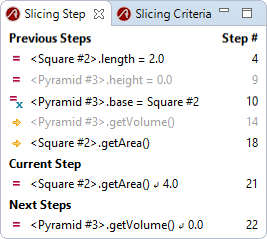
\includegraphics[width=0.60\textwidth]{slice1.png}
	\caption{The slice navigator view, for the program halted at \linerefn{lst:example}{6}.}
	\label{fig:slice1}
\end{figure}

Using this event list, the developer can obtain different kinds of information about the current state of the execution.
Firstly, simply by looking at the previous and next steps, the developer can understand at a glace how the current instruction fits into the grander scheme.
This is particularly useful if the current instruction was reached via a breakpoint, in which case it is not always obvious at which point in time it was hit.
To obtain this kind of information with a regular debugger, the developer needs to analyze the execution stack and maybe even inspect lower stack frames.

Secondly, it provides a summary of the program state.
Unlike a typical debugger's variable view, the slice navigator only shows relevant variables, and also shows relevant object fields on the first level.
Furthermore, the developer can easily investigate the origin of a value.
Simply clicking an event moves the execution to that point in time.
This way, the slice navigator allows to efficiently follow infection chains of erroneous state.

Thirdly, the slice navigator shows details about the dependency graph that was used to compute the current slice.
Small icons indicate how the events of the slice are related.
The next section explains how again the navigator serves not only as a visualization, but also allows the developer to interact with the underlying tools.

\subsection{Interactive Slice Configuration}

The slicing component is based on previous work \todo{[xxx]}.
When building the dependency graph between events, the algorithm distinguishes between three types of dependencies.
\emph{Value dependencies} occur when the the value of an instruction is derived from another instruction's value.
In the slice navigator, they are represented with a red equality sign.
Instructions that determine if another instruction can be reached are \emph{reachability dependencies}, indicated by a yellow arrow.
Typically, these are method invocations and instruction in conditional statements.
Sometimes, a value depends on only one of multiple candidate values. 
A \emph{control dependency} determines which of these candidates is used.
More formally, control dependencies are reachability dependencies of value candidates that are not also reachability dependencies of all other candidates.
In the navigator, they are indicated by a blue "X".

The developer can now combine these different dependency types to adjust the slice for specific purposes.
Clicking on an event's dependency symbol brings up a dialog that allows to choose which dependencies of that event to include.
This way the developer can, for instance, put a focus on how a value was computed or how an instruction was reached.
It is also possible to remove all dependencies of an event, for instance if it is known to be correct and its history is not of interest, thereby moving the focus of the slice to less well-understood parts of the program.

\begin{figure}
	\centering
		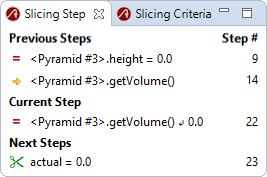
\includegraphics[width=0.60\textwidth]{slice2.png}
	\caption{The program halted at \linerefn{lst:example}{21}, after \lstinline{getArea()} was removed from the slice.}
	\label{fig:slice2}
\end{figure}

Whenever a slicing criterion is modified, the slice is updated instantly, without locking the user interface or resetting the current debug session.
In our examples, the developer might choose to exclude the result of ´getArea()´ from the slice. 
As shown in \cref{fig:slice2}, with the computation of the area removed from the slice it is now much easier to see that the wrong result of ´getVolume()´ was caused by a wrong value in ´height´.


As mentioned before, instructions and states not belonging to the slice are still shown in the IDE, mostly to serve as an orientation help, to provide context to the current operations.
However, it might also happen that a value or instruction outside of the slice catches the developers attention.
In this case, she can choose to add it as another slicing criterion and the slice is immediately expanded.
Again, this happens without interrupting the developer's work.
In the worst case, expanding the slice takes as long as creating a new slice for only that event.
The developer might notice how new events are added to the slice in the background.
Generally, this should not be an impediment, as events that are closest to the current instruction are added first.

\section{Implementation}
\label{sec:impl}

The slice navigator is part of a set of debugging tools that are implemented as an Eclipse plug-in.

\subsection{Framework}

The high-level architecture of our prototype consists of three components: the tracer, the event database, and the omniscient debugger with the slicing module.

The tracer is implemented as a Java agent that modifies the bytecode of a program to insert tracing instructions that log all events into csv files.
With our Eclipse plug-in, the developer can initiate an omniscient debug session by selecting a customized launcher in the run configuration.
The launcher will add VM arguments to the execution to configure the tracer.
Once the execution completes, the launcher will automatically import the trace data into the configured database.
We provide launchers for basic Java applications and for JUnit test suites.
For JUnit launches, the tracer will treat each test case as an independent execution and ignore code of the testing framework.

The database stores all events of a set of executions.
It is possible to set up one database per project or one for the entire workspace.
We currently support HSQLDB, MySql, and SAP Hana, but in principle any relational database can be used.

The omniscient debugger consists of a set of views that allow to debug a Java application based on the data from the database.
It is a post-mortem debugger, i.e., it simulates a debug session while the actual program has already terminated.

\subsection{Slicing algorithm}

\todo{The slicing component is based on previous work [xxx].}
The basic structure is of the slicing algorithm is fairly simple and shown in \cref{lst:slicealgo}.

\begin{lstlisting}[numberfirstline=true,float,language=algorithm,firstnumber=1,label=lst:slicealgo,caption={Algorithm for building the slice}]
	function build_slice(criteria)
		slice := {}
		for each event \in criteria do ''in parallel''
			add_to_slice(slice, event)
		return slice
		
	function add_to_slice(slice, event)
	  if event \in slice || event.is_negative_criterion then return
		'add' event 'to' slice
		static_dependency_graph := event.method.dependency_graph
		static_dependencies := static_dependency_graph.get(event.instruction)
		for each instruction \in static_dependencies do ''in parallel''
			prev_event := find_last_previous_event(instruction)
			if prev_event 'exists' then
				add_to_slice(slice, prev_event)
\end{lstlisting}

%\begin{lstlisting}[numberfirstline=true,language=algorithm,firstnumber=1,label=lst:slicealgo,caption={Example program with a failing test case}]
	%function build_slice(criteria)
		%slice := {}
		%for each event \in criteria do ''in parallel''
			%add_to_slice(slice, event)
		%return slice
		%
	%function add_to_slice(slice, event)
		%'add event to slice'
		%'get static dependency graph of event\'s method'
		%'get static dependencies of event\'s instruction'
		%for each instruction \in 'static dependencies' do ''in parallel''
			%'find last previous event at instruction'
			%if 'previous event exists' && 'previous event' \notin slice then
				%add_to_slice(slice, 'previous event')
%\end{lstlisting}

%A static code analysis built with the Soot framework creates static dependency graphs on the method level.
%Static dependency graphs are computed on demand and cached for reuse.

The slicing criterion is a set of events, the slice is initially an empty set.
For each event that is added to the slice, the static dependency graph of the event's method is obtained.
If the graph is not initialized yet, it will be created by a code analysis using the Soot framework.
The dependency graph contains every instruction's static dependencies and distinguishes between three dependency types, as described in the previous section.
Dependency instruction candidates are looked up in the graph by the event's instruction.

For each candidate instruction, the latest occurrence is looked up in the event database.
For variable assignments the look up is limited to the current method invocation, for events like field assignments the scope is not limited.
If an event was found, it will be added to the slice next.


%soot-based analysis for static dependency graph, cached as needed\\
%for every event: map to statement, find dependency statements, map to event\\
%improved user exp: intermediate result twice per second.\\

%The slice configuration contains two kind of information.
%First, the slicing criterion, which is a list of initial events.




%if event is encountered, only configured dependency types are followed\\
  %if none configured, configuration is inherited\\
  %on multi inheritance, flags are `or`-ed.\\
  %changes are propagated to previous events\\
  %
%due to parallel nature of algorithm, change via user or algorithm similar \\
%except user may remove dependency types\\
%after a change, dependencies are added or removed accordingly\\
%on remove, reference counting to decide if event is removed entirely\\

\section{Evaluation}
\label{sec:eval}

performance\\

example\\

\section{Conclusion}
\label{sec:conclusion}


\printbibliography

\end{document}